\chapter{Organogênese: a formação do membro dos tetrápodes}\label{ch:b2:limb-organogenesis}

Três dias depois que um ovo de galinha é posto, uma saliência do
tamanho de uma cabeça de alfinete aparece em cada flanco do embrião.
Quatro dias depois, ela é uma asa, com um úmero, um rádio e uma ulna,
um punho e três dedos, na ordem certa, nos comprimentos certos, com os
músculos presos aos ossos certos. Retire a borda de pele espessada da
saliência e a asa para de crescer; enxerte uma lasca de sua margem
posterior em sua margem anterior e ela forma seis dedos em imagem
especular. O \omterm{def:b2:limb-organogenesis:bud}{broto do membro} é o caso clássico de
\emph{organogênese} --- a construção de um órgão a partir de um campo
de células por sinais que dizem a que distância para fora, para a
frente e para cima cada célula está ---, e os experimentos que o
decifraram estão entre os mais claros da biologia. Este capítulo
acompanha o broto desde seu crescimento até seu esqueleto.

\section{O broto e seus três eixos}

\begin{definition}[O broto do membro]\label{def:b2:limb-organogenesis:bud}
\index{broto do membro}\index{crista ectodérmica apical}\index{zona de atividade polarizante}
O \emph{broto do membro} é uma saliência de \emph{mesoderma da placa
lateral} recoberta de ectoderma, que surge numa posição fixa ao longo
do flanco (o \emph{campo do membro}) onde o código Hox do eixo corporal
o permite; seu mesoderma formará osso, cartilagem, tendão e derme, e as
células que migram para ele a partir dos somitos formarão os músculos.
O broto tem três eixos, cada um comandado por um centro sinalizador.
\emph{Proximodistal} (do ombro à ponta dos dedos): a \emph{crista
ectodérmica apical} (AER), uma faixa espessada de ectoderma ao longo da
ponta, secreta \omterm{prop:b2:limb-organogenesis:aer}{fatores de crescimento de fibroblastos} (FGFs) que
mantêm o mesoderma subjacente em divisão e indiferenciado.
\emph{Anteroposterior} (do polegar ao dedo mínimo): a \emph{zona de
atividade polarizante} (ZPA), um bloco de mesoderma na margem
posterior, secreta o morfógeno \emph{\omterm{prop:b2:limb-organogenesis:zpa}{Sonic hedgehog}} (Shh).
\emph{Dorsoventral} (do dorso da mão à palma): o ectoderma dorsal
secreta Wnt7a. Os brotos dos membros anteriores e posteriores se
parecem e usam os mesmos sinais; eles diferem por um fator de
transcrição expresso antes do aparecimento do broto (Tbx5 no membro
anterior, Tbx4 no posterior), e é por isso que uma asa é uma asa.
\end{definition}

\begin{omfigure}
\begin{tikzpicture}[every node/.style={font=\scriptsize}, >=stealth]
  % flank
  \fill[omExo!25] (0,-2.2) rectangle (1.2,2.2); \node[rotate=90] at (0.6,0) {parede do corpo (flanco)};
  % bud outline: paddle
  \draw[thick, fill=omDef!10] (1.2,1.4) .. controls (3.0,1.9) and (5.2,1.6) .. (5.8,0.3) .. controls (5.9,-0.3) and (5.2,-1.6) .. (3.4,-1.7) .. controls (2.4,-1.8) and (1.6,-1.5) .. (1.2,-1.4);
  % AER along the tip
  \draw[line width=3pt, omThm] (5.2,1.3) .. controls (5.9,0.6) and (5.9,-0.6) .. (5.0,-1.4);
  \node[omThm, anchor=west, align=left] at (6.1,0.9) {crista ectodérmica apical (AER):\\FGFs, crescimento proximodistal};
  % ZPA posterior
  \draw[thick, omProp, fill=omProp!50] (2.4,-1.1) ellipse (0.55 and 0.4);
  \draw[omProp] (2.4,-1.5) -- (2.4,-2.0);
  \node[omProp, anchor=north, align=center] at (2.6,-2.0) {ZPA (margem posterior):\\Sonic hedgehog, anteroposterior};
  % dorsal ectoderm
  \draw[line width=2pt, omDef!70!black] (1.4,1.55) .. controls (3.0,2.0) and (5.0,1.7) .. (5.4,1.2);
  \node[omDef!70!black, anchor=south] at (3.4,2.05) {ectoderma dorsal: Wnt7a, dorsoventral};
  % axes
  \draw[->, thick] (1.5,-3.1) -- (5.5,-3.1); \node[below] at (3.5,-3.15) {proximal $\to$ distal};
  \draw[->, thick] (10.6,-1.6) -- (10.6,1.2); \node[right, align=left] at (10.7,-0.2) {posterior $\to$ anterior\\(do dedo mínimo ao polegar)};
\end{tikzpicture}

{\small O \omterm{def:b2:limb-organogenesis:bud}{broto do membro} da galinha visto de cima, com seus três
centros sinalizadores: a AER, ao longo da ponta, comanda o crescimento;
a ZPA, na margem posterior, padroniza os dedos; o ectoderma dorsal
distingue o dorso da palma.}
\end{omfigure}

\begin{omfigure}
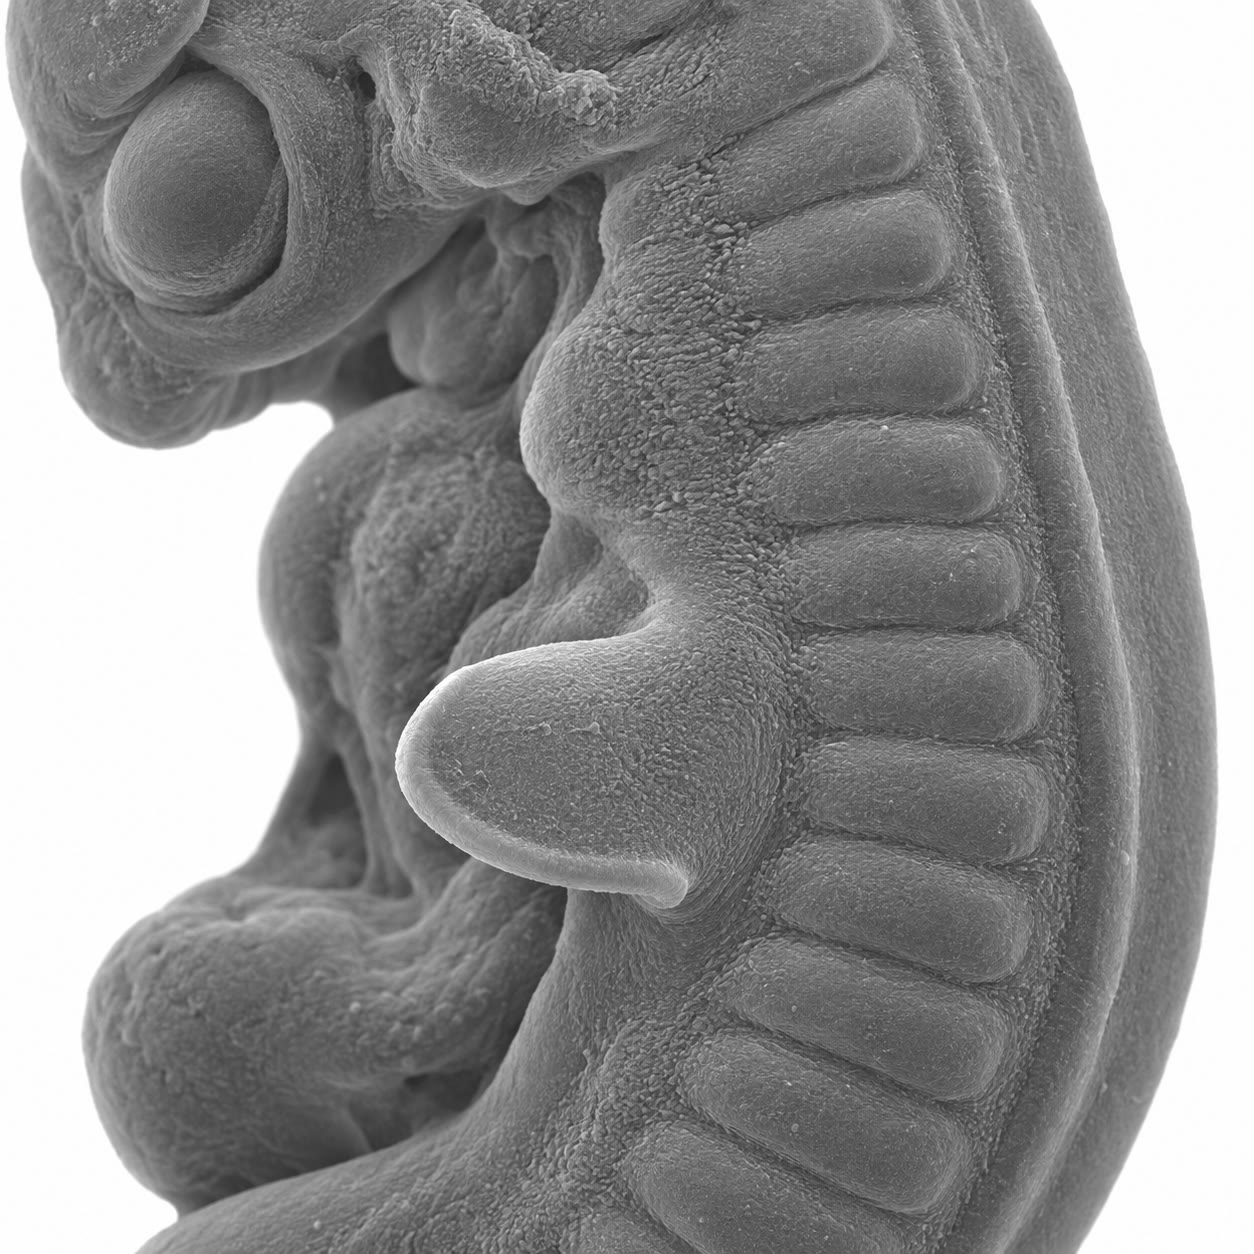
\includegraphics[width=0.42\linewidth]{images/book4/ai/b4-11-limb-bud.jpg}

{\small Um embrião de galinha ao microscópio eletrônico de varredura: a
fileira de somitos ao longo do tronco e, no flanco, o \omterm{def:b2:limb-organogenesis:bud}{broto do membro}
em forma de remo, com a crista espessada ao longo da borda.}
\end{omfigure}

\section{O crescimento: o eixo proximodistal}

\begin{proposition}[A crista ectodérmica apical]\label{prop:b2:limb-organogenesis:aer}
\index{fator de crescimento de fibroblastos}\index{zona de progresso}
A AER é necessária para o crescimento, e seus FGFs são suficientes: o
mesoderma sob ela, a \emph{\omterm{prop:b2:limb-organogenesis:aer}{zona de progresso}}, se divide a cada doze
horas, mais ou menos, e as células que deixam a zona à medida que a
ponta avança param de se dividir, se condensam e se diferenciam. O
esqueleto se forma em ordem proximodistal --- \emph{estilopódio} (úmero
ou fêmur), \emph{zeugopódio} (rádio e ulna, tíbia e fíbula),
\emph{autopódio} (punho e dedos) ---, cada segmento especificado por sua
vez à medida que o broto cresce, e os segmentos correspondem a domínios
encaixados de expressão de genes Hox (Hoxa/d 9--10 no estilopódio, 11
no zeugopódio, 13 no autopódio). Um broto de membro cresce cerca de dez
vezes em comprimento em quatro dias, enquanto o alcance do sinal da
crista permanece nas mesmas poucas centenas de micrômetros, de modo que
a crista padroniza o membro não de uma vez, mas como uma frente em
movimento, do modo como uma impressora imprime uma página linha por
linha.
\end{proposition}
\begin{proof}[Evidências]
Saunders (1948) removeu a AER de brotos de asa de galinha em estágios
sucessivos: removida cedo, o broto dava apenas um coto de úmero;
removida um dia depois, úmero e antebraço, mas nenhuma mão; removida
mais tarde ainda, uma asa quase completa --- quanto mais tardia a
operação, mais distal o nível de truncamento, de modo que a crista é
necessária para cada segmento por sua vez. Enxertar uma segunda crista
produzia um segundo crescimento; uma microesfera embebida em FGF,
colocada num broto cuja crista fora removida, restaurava um membro
completo (Niswander, 1993), e uma microesfera colocada no flanco, entre
os campos dos membros, induzia um membro extra. Os camundongos sem os
FGFs da crista não têm membros.
\end{proof}

\begin{omfigure}
\begin{tikzpicture}[every node/.style={font=\scriptsize}]
  \foreach \x/\lab/\n in {0/{AER removida cedo:\\só o úmero}/1, 3.6/{removida um dia depois:\\úmero, rádio, ulna}/2, 7.2/{removida mais tarde:\\asa quase completa}/3, 10.8/{intacta:\\asa completa}/4} {
    \begin{scope}[xshift=\x cm]
      \fill[omExo!25] (0,-0.5) rectangle (0.5,2.6);
      % humerus
      \draw[thick, fill=omDef!25, rounded corners=3pt] (0.6,0.9) rectangle (1.7,1.2);
      \ifnum\n>1 \draw[thick, fill=omDef!25, rounded corners=3pt] (1.8,1.05) rectangle (2.7,1.3); \draw[thick, fill=omDef!25, rounded corners=3pt] (1.8,0.75) rectangle (2.7,1.0); \fi
      \ifnum\n>2 \foreach \y in {0.55,0.85,1.15} \draw[thick, fill=omDef!25, rounded corners=2pt] (2.8,\y) rectangle (3.3,\y+0.2); \fi
      \ifnum\n=4 \foreach \y in {0.55,0.85,1.15} \draw[thick, fill=omDef!25, rounded corners=2pt] (3.35,\y) rectangle (3.5,\y+0.2); \fi
      \node[below, align=center] at (1.8,-0.2) {\lab};
    \end{scope}
  }
\end{tikzpicture}

{\small O experimento de Saunders. Quanto mais cedo a crista é
removida, maior a parte do membro que falta, sempre a partir da ponta:
a crista é necessária para cada segmento enquanto ele está sendo
formado.}
\end{omfigure}

\begin{theorem}[Crescimento por divisão]\label{thm:b2:limb-organogenesis:growth}
Um broto cujas células se dividem a cada $T$ horas multiplica seu
número de células por $2^{t/T}$ num tempo $t$; quatro dias de ciclos de
doze horas dão
$2^{8} = 256$. Se o volume do broto cresce mil vezes nesses quatro
dias, a divisão fornece um fator de 256, e o fator restante, de quatro,
precisa vir do aumento das células e da matriz que as células da
cartilagem secretam em torno de si. Inversamente, um segmento que leva
um ciclo celular para ser especificado --- as cerca de doze horas que
separam os níveis de truncamento sucessivos do experimento de Saunders
--- corresponde a uma duplicação da \omterm{prop:b2:limb-organogenesis:aer}{zona de progresso}.
\end{theorem}
\begin{proof}
$N(t) = N_0 2^{t/T}$; com $t = \qty{96}{h}$ e $T = \qty{12}{h}$,
$t/T = 8$. A razão entre o fator necessário e o fator de divisão,
$1000/256 \approx 4$, é o que o crescimento, além da divisão, precisa
fornecer.
\end{proof}

\section{Os dedos: o eixo anteroposterior}

\begin{proposition}[A zona de atividade polarizante]\label{prop:b2:limb-organogenesis:zpa}
\index{Sonic hedgehog}\index{morfógeno!Shh}
A ZPA especifica que dedo se forma em cada lugar. Suas células secretam
\omterm{prop:b2:limb-organogenesis:zpa}{Sonic hedgehog}, que se espalha pelo broto a partir da margem posterior,
e as células do mesoderma leem a concentração --- e o tempo durante o
qual foram expostas a ela --- como uma posição: a dose mais alta dá o
dedo mais posterior, doses mais baixas dão dedos mais anteriores, e
abaixo de um limiar não se forma dedo algum. O gradiente tem a forma
exponencial do \cref{ch:b2:vertebrate-development}, com um comprimento de decaimento de algumas
dezenas de micrômetros, e seus limiares dividem o broto nos primórdios
dos dedos: na asa da galinha, de trás para a frente, os dedos 4, 3 e
2. Uma segunda fonte do sinal na margem anterior produz um segundo
conjunto, em imagem especular; uma fonte mais fraca, ou uma exposição
mais curta, produz apenas os dedos anteriores do conjunto extra. O
mesmo gene, no mesmo papel, padroniza os dedos de todos os tetrápodes,
e uma \omterm{def:b2:genome-diversification:mutation}{mutação} que acrescenta uma fonte anterior de Shh causa
polidactilia em gatos, galinhas, camundongos e seres humanos.
\end{proposition}
\begin{proof}[Evidências]
Saunders e Gasseling (1968) enxertaram um bloco de mesoderma da margem
posterior de um broto de asa de galinha na margem anterior de outro: o
hospedeiro formou uma asa com seis dedos na ordem 4-3-2-2-3-4, uma
imagem especular em relação ao meio. Tickle (1975) mostrou que o número
de dedos extras dependia do número de células enxertadas --- uma dose.
Riddle e Tabin (1993) descobriram que o tecido enxertado expressava o
gene \emph{\omterm{prop:b2:limb-organogenesis:zpa}{Sonic hedgehog}}, que o gene não era expresso em nenhum outro
ponto do broto, e que células modificadas para expressá-lo, enxertadas
na margem anterior, reproduziam a duplicação especular; uma
microesfera da proteína fazia o mesmo. Mutantes de galinha com uma
mancha ectópica anterior de Shh têm dedos anteriores extras.
\end{proof}

\begin{omfigure}
\begin{tikzpicture}[every node/.style={font=\scriptsize}, >=stealth]
  % normal bud with gradient and digits
  \begin{scope}
    \fill[omExo!25] (0,-0.3) rectangle (0.4,3.3);
    \shade[bottom color=omProp!60, top color=white] (0.4,-0.3) rectangle (3.2,3.3);
    \draw[thick] (0.4,-0.3) rectangle (3.2,3.3);
    \draw[thick, omProp, fill=omProp!70] (0.9,0.1) ellipse (0.45 and 0.35); \node[omProp!80!black, anchor=west] at (1.4,0.1) {ZPA};
    \foreach \y/\d in {0.6/4, 1.5/3, 2.4/2} { \draw[thick, fill=omDef!25, rounded corners=2pt] (3.3,\y-0.12) rectangle (4.2,\y+0.12); \node[right] at (4.25,\y) {dedo \d}; }
    \node[below, align=center] at (2.0,-0.5) {broto normal: Shh a partir da\\margem posterior, dedos 4-3-2};
    \draw[->, thick] (-0.4,0.2) -- (-0.4,3.0); \node[rotate=90] at (-0.7,1.6) {posterior $\to$ anterior};
  \end{scope}
  % grafted bud
  \begin{scope}[xshift=7cm]
    \fill[omExo!25] (0,-0.3) rectangle (0.4,3.3);
    \shade[bottom color=omProp!60, top color=white] (0.4,-0.3) rectangle (3.2,1.5);
    \shade[top color=omProp!60, bottom color=white] (0.4,1.5) rectangle (3.2,3.3);
    \draw[thick] (0.4,-0.3) rectangle (3.2,3.3);
    \draw[thick, omProp, fill=omProp!70] (0.9,0.1) ellipse (0.45 and 0.35);
    \draw[thick, omProp, fill=omProp!70] (0.9,2.9) ellipse (0.45 and 0.35); \node[omProp!80!black, anchor=west] at (1.4,2.9) {ZPA enxertada};
    \foreach \y/\d in {0.3/4, 0.8/3, 1.3/2, 1.7/2, 2.2/3, 2.7/4} { \draw[thick, fill=omDef!25, rounded corners=2pt] (3.3,\y-0.1) rectangle (4.2,\y+0.1); \node[right] at (4.25,\y) {\d}; }
    \node[below, align=center] at (2.0,-0.5) {ZPA enxertada na margem anterior:\\duplicação especular 4-3-2-2-3-4};
  \end{scope}
\end{tikzpicture}

{\small A região polarizante. À esquerda: o Shh se espalha a partir da
margem posterior, e sua concentração decrescente especifica os dedos
4, 3 e 2. À direita: uma segunda ZPA enxertada na margem anterior cria
um segundo gradiente e um conjunto de dedos em imagem especular.}
\end{omfigure}

\begin{theorem}[Fronteiras dos dedos a partir do gradiente]\label{thm:b2:limb-organogenesis:thresholds}
Com o Shh à concentração $c_0$ na margem posterior e um comprimento de
decaimento $\lambda$, a fronteira do território de um dedo cujo limiar
é $T_i$ fica a $x_i = \lambda\ln(c_0/T_i)$ da margem. Com
$\lambda = \qty{50}{\micro m}$ e limiares de $0.6$,
$0.25$ e $0.08$ de $c_0$ para os dedos 4, 3 e 2, os territórios vão de
$0$--$26$, $26$--$69$ e $69$--$126$ micrômetros, e o tecido além de
\qty{126}{\micro m} não forma dedo. Dobrar a fonte desloca todas as
fronteiras para fora em $\lambda\ln 2 = \qty{35}{\micro m}$ --- o
bastante, num broto de algumas centenas de micrômetros, para
acrescentar um dedo na borda anterior; uma segunda fonte na margem
anterior dispõe os mesmos territórios em ordem inversa.
\end{theorem}
\begin{proof}
A partir de $c(x) = c_0 e^{-x/\lambda}$, $c = T_i$ em $x_i = \lambda
\ln(c_0/T_i)$: $50\ln(1/0.6) = 25.5$, $50\ln 4 = 69$, $50\ln 12.5 =
126$. Substituir $c_0$ por $2c_0$ acrescenta $\lambda\ln 2$ a cada
$x_i$.
\end{proof}

\begin{omfigure}
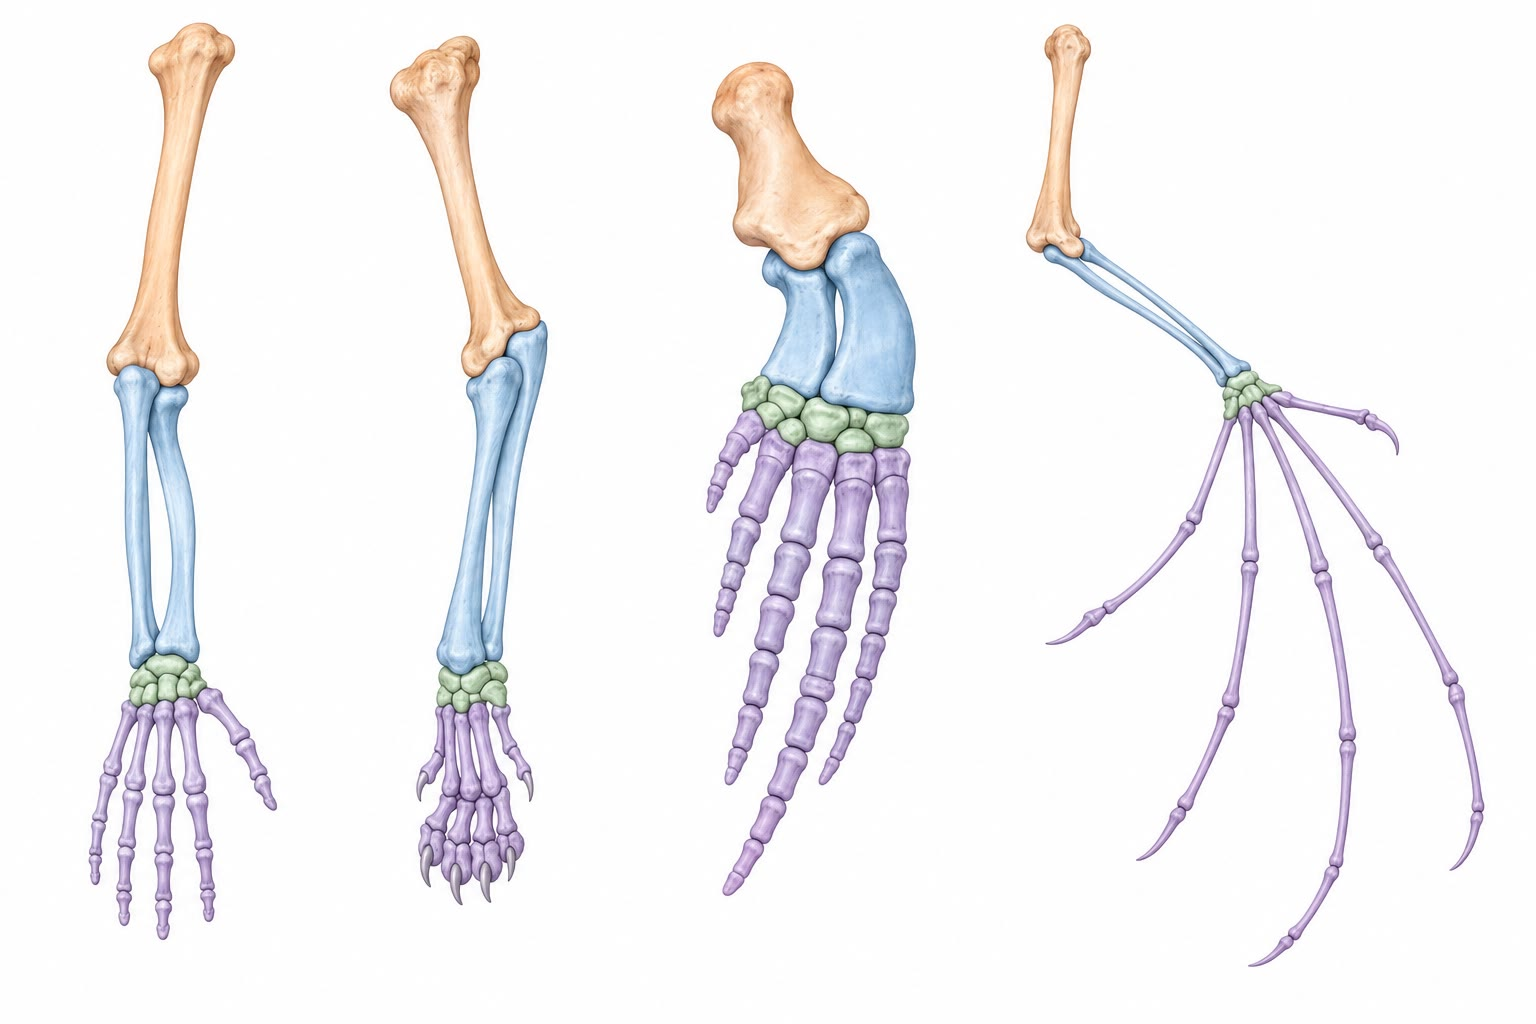
\includegraphics[width=0.66\linewidth]{images/book4/ai/b4-11-tetrapod-limbs.jpg}

{\small Um plano, quatro membros: os membros anteriores de um ser
humano, de um gato, de uma baleia e de um morcego compartilham os
mesmos ossos na mesma ordem --- um estilopódio, dois ossos do
zeugopódio, punho, dedos ---, construídos pelos mesmos centros
sinalizadores e diferentes no crescimento.}
\end{omfigure}

\section{Coordenação e modelagem}

\begin{proposition}[Os eixos conversam entre si]\label{prop:b2:limb-organogenesis:loop}
\index{alça de retroalimentação!no desenvolvimento}
Os centros mantêm uns aos outros: o FGF da crista mantém a ZPA
expressando Shh, e o Shh, por meio de um revezamento no mesoderma,
mantém a crista expressando FGF; retire um dos dois e o outro se
extingue em um dia. O Wnt7a do ectoderma dorsal também é necessário
para a expressão plena do Shh, e comanda o destino dorsal do mesoderma
(um camundongo sem ele tem duas palmas). Essa dependência mútua é uma
\emph{alça de retroalimentação positiva} que trava os três eixos
juntos: o membro só cresce onde está sendo padronizado e só é
padronizado onde está crescendo, de modo que um broto nunca forma uma
mão sem braço, nem dedos do tipo errado. Quando o crescimento termina,
a alça se rompe --- o mesoderma para de fazer o revezamento, o Shh
cessa, a crista regride --- e o membro para de crescer no tamanho
adequado.
\end{proposition}

\begin{proposition}[Do padrão ao osso]\label{prop:b2:limb-organogenesis:skeleton}
\index{condrogênese}\index{apoptose!interdigital}
Uma vez especificadas, as células do mesoderma que deixam a \omterm{prop:b2:limb-organogenesis:aer}{zona de
progresso} se \emph{condensam} em bastões e placas com a forma dos
futuros ossos, diferenciam-se em células de cartilagem que secretam uma
matriz rica em colágeno e proteoglicanos, e depositam um modelo
cartilaginoso de cada elemento do esqueleto; as articulações se formam
onde uma faixa de células recebe a instrução de não se tornar
cartilagem; vasos sanguíneos invadem os modelos e o osso substitui a
cartilagem do centro para as extremidades, deixando nas pontas placas
de crescimento que mantêm o osso se alongando até a idade adulta
(\emph{ossificação endocondral}). Precursores musculares vindos dos
somitos migram para dentro, se dividem, se fundem em fibras
(\cref{ch:b2:cell-differentiation}) e se prendem por tendões formados pelo próprio mesoderma do
membro. Entre os raios dos dedos, o tecido é eliminado por morte
celular programada: as células das membranas interdigitais, sob o sinal
de uma proteína morfogenética óssea (BMP), ativam sua própria
destruição e são removidas em um dia, o que separa os dedos. Um pato
conserva suas membranas porque um inibidor de BMP é expresso em seu
tecido interdigital; uma galinha que recebe o mesmo inibidor numa
microesfera desenvolve pés palmados.
\end{proposition}
\begin{proof}[Evidências]
Mesoderma interdigital retirado de um broto de perna de galinha e
enxertado em outro lugar morre no prazo previsto --- a morte é
intrínseca, decidida antes da retirada do tecido; o mesmo tecido
retirado de um pato sobrevive. Microesferas de BMP colocadas entre os
dedos de um pato fazem a membrana morrer; microesferas do inibidor
gremlin colocadas entre os dedos de uma galinha a salvam. Um
camundongo sem um receptor de BMP no membro conserva as membranas.
\end{proof}

\begin{omfigure}
\begin{tikzpicture}[every node/.style={font=\scriptsize}]
  \foreach \x/\lab in {0/{os raios dos dedos se\\condensam em cartilagem}, 4.2/{as células interdigitais\\morrem (BMP)}, 8.4/{dedos separados;\\o osso substitui a cartilagem}} {
    \begin{scope}[xshift=\x cm]
      \node[below, align=center] at (1.5,-0.3) {\lab};
    \end{scope}
  }
  % stage 1: paddle with rays
  \draw[thick, fill=omDef!8] (0,0) .. controls (0,2.2) and (3,2.2) .. (3,0) -- cycle;
  \foreach \x in {0.6,1.2,1.8,2.4} \draw[thick, fill=omDef!30, rounded corners=2pt] (\x-0.12,0.1) rectangle (\x+0.12,1.5);
  % stage 2: paddle with dying webs
  \begin{scope}[xshift=4.2cm]
    \draw[thick, fill=omDef!8] (0,0) .. controls (0,2.2) and (3,2.2) .. (3,0) -- cycle;
    \foreach \x in {0.6,1.2,1.8,2.4} \draw[thick, fill=omDef!30, rounded corners=2pt] (\x-0.12,0.1) rectangle (\x+0.12,1.5);
    \foreach \x in {0.9,1.5,2.1} \foreach \y in {0.7,1.0,1.3} \fill[omThm] (\x,\y) circle (0.05);
  \end{scope}
  % stage 3: separated digits
  \begin{scope}[xshift=8.4cm]
    \draw[thick, fill=omDef!8] (0,0) -- (0,0.5) -- (0.3,0.5) -- (0.35,1.7) -- (0.85,1.7) -- (0.9,0.5) -- (1.05,0.5) -- (1.1,1.85) -- (1.6,1.85) -- (1.65,0.5) -- (1.8,0.5) -- (1.85,1.7) -- (2.35,1.7) -- (2.4,0.5) -- (2.7,0.5) -- (2.7,0) -- cycle;
    \foreach \x in {0.6,1.35,2.1} \draw[thick, fill=omExo!60, rounded corners=2pt] (\x-0.1,0.1) rectangle (\x+0.1,1.4);
  \end{scope}
\end{tikzpicture}

{\small A modelagem da mão: raios de cartilagem se condensam no remo,
as células entre eles morrem (vermelho) e os dedos liberados se
ossificam.}
\end{omfigure}

\begin{example}[O mesmo membro, crescido de outro modo]\label{ex:b2:limb-organogenesis:evolution}
A asa do morcego é uma mão cujos dedos 2 a 5 cresceram várias vezes
mais que os de um camundongo --- um intensificador de um gene do membro,
transplantado do morcego para o camundongo, alonga os ossos do membro
anterior do camundongo --- e cujo tecido interdigital sobreviveu,
porque a membrana expressa o inibidor de BMP que o pato usa. A
nadadeira da baleia é uma mão com falanges extras e sem morte
interdigital. A perna do cavalo é um único dedo, com os outros
reduzidos a estiletes. A serpente não tem membros porque seu flanco
nunca expressa os sinais que iniciam um broto. E as nadadeiras dos
peixes, que não têm autopódio, são construídas pelas mesmas AER e ZPA,
mas interrompem seu programa Hox antes da fase tardia que forma os
dedos; o fóssil \emph{Tiktaalik} (375 milhões de anos) mostra o punho
aparecendo numa nadadeira. A evolução dos membros é sobretudo a
modulação de um programa conservado --- quanto tempo dura cada fase,
até onde chega cada sinal, que células morrem.
\end{example}

\section{Exercícios}

\begin{exercise}[$\star$]\label{exo:b2:limb-organogenesis:1}
Cite os três eixos do \omterm{def:b2:limb-organogenesis:bud}{broto do membro} e, para cada um, o centro
sinalizador, sua posição e seu sinal.
\end{exercise}

\begin{exercise}[$\star$]\label{exo:b2:limb-organogenesis:2}
Dê os três segmentos do esqueleto do membro e os ossos de cada um no
braço e na perna humanos. Que genes Hox os marcam?
\end{exercise}

\begin{exercise}[$\star$]\label{exo:b2:limb-organogenesis:3}
Liste, em ordem, as etapas que levam de uma mancha de mesoderma da
placa lateral a um dedo com seu osso, sua articulação e seu músculo.
\end{exercise}

\begin{exercise}[$\star$]\label{exo:b2:limb-organogenesis:4}
Como fica o membro se a AER for removida (a) assim que o broto
aparece, (b) depois que o antebraço foi especificado, (c) não removida,
mas substituída por uma microesfera de FGF?
\end{exercise}

\begin{exercise}[$\star\star$]\label{exo:b2:limb-organogenesis:5}
Com $\lambda = \qty{40}{\micro m}$ e limiares de $0.5$, $0.2$
e $0.05$ da concentração na fonte para os dedos 4, 3 e 2, calcule as
três fronteiras e a largura do território de cada dedo.
\end{exercise}

\begin{exercise}[$\star\star$]\label{exo:b2:limb-organogenesis:6}
Preveja o padrão dos dedos de uma asa de galinha após (a) uma ZPA
inteira enxertada na margem anterior, (b) um enxerto com um quarto das
células da ZPA, (c) uma microesfera de Shh na margem anterior, retirada
após uma exposição curta. Explique cada caso pela dose e pelo tempo.
\end{exercise}

\begin{exercise}[$\star\star$]\label{exo:b2:limb-organogenesis:7}
Um broto de membro de galinha tem \num{5000} células quando a crista se
forma, e suas células se dividem a cada \qty{12}{h}. Quantas células
há após quatro dias? Se o membro tem, nesse estágio, $4\times 10^{6}$
células, o que precisa ser verdade sobre o ciclo celular ou sobre a
morte celular?
\end{exercise}

\begin{exercise}[$\star\star$]\label{exo:b2:limb-organogenesis:8}
Explique por que uma galinha tem dedos livres e um pato pés palmados, e
o que faz uma microesfera de inibidor de BMP entre os dedos de um
embrião de galinha. O que o momento intrínseco da morte interdigital
(ela ocorre no prazo previsto num enxerto) diz sobre o modo como as
células foram instruídas?
\end{exercise}

\begin{exercise}[$\star\star$]\label{exo:b2:limb-organogenesis:9}
Um camundongo não tem nem Hoxa13 nem Hoxd13; outro não tem Hoxa11 nem
Hoxd11. Preveja o esqueleto de cada membro anterior e diga o que o
resultado mostra sobre a relação entre os domínios Hox e os segmentos.
\end{exercise}

\begin{exercise}[$\star\star\star$]\label{exo:b2:limb-organogenesis:10}
Explique a retroalimentação positiva entre a AER e a ZPA, por que ela
torna o membro robusto, e o que aconteceria com um broto em que o Shh
não conseguisse manter o FGF. Compare-a com a retroalimentação positiva
do trabalho de parto no \cref{ch:b2:mammal-reproduction}: o que encerra cada alça?
\end{exercise}

\begin{exercise}[$\star\star\star$]\label{exo:b2:limb-organogenesis:11}
O terceiro dedo de um morcego é oito vezes mais longo que o de um
camundongo em relação ao tamanho do corpo. Se a cartilagem do dedo se
alonga exponencialmente à taxa $r$ por dia durante uma janela de
crescimento, e a janela do morcego é quatro dias mais longa que a do
camundongo, que $r$ é necessário? Dê duas modificações do
desenvolvimento (uma no crescimento, uma na morte celular) que fazem
de uma mão uma asa.
\end{exercise}

\begin{exercise}[$\star\star\star$]\label{exo:b2:limb-organogenesis:12}
O \omterm{prop:b2:limb-organogenesis:zpa}{Sonic hedgehog} padroniza o \omterm{prop:b2:vertebrate-development:neurulation}{tubo neural} a partir da placa do assoalho
(\cref{ch:b2:vertebrate-development}) e os dedos a partir da ZPA. Discuta por que a evolução
reutiliza poucos sinais para muitas tarefas, como a mesma molécula pode
significar coisas diferentes em tecidos diferentes, e o que isso
implica para o efeito de uma \omterm{def:b2:genome-diversification:mutation}{mutação} num gene desse tipo.
\end{exercise}

\section{Problema: Uma asa construída em uma semana}

\begin{problem}[{Problema de fim de semana --- a asa da galinha
acompanhada do broto ao esqueleto: seu crescimento por divisão, as
remoções da crista de Saunders cronometradas, o gradiente de Shh
calculado e suas duplicações previstas, as membranas modeladas e a asa
comparada com a de um morcego, até o número de duplicações, as
fronteiras dos dedos e a largura de que um broto precisa para uma
duplicação especular}]
\label{pb:b2:limb-organogenesis:1}
Um broto de asa de galinha aparece com 3 dias de incubação, com
\num{2000} células de mesoderma e um comprimento de \qty{0.4}{mm}; aos
7 dias, a asa tem \qty{4}{mm} de comprimento e seu volume é \num{1000}
vezes o do broto. As células da \omterm{prop:b2:limb-organogenesis:aer}{zona de progresso} se dividem a cada
\qty{12}{h}. Remoções da crista: aos 3.0 dias, o membro é um coto; aos
3.5 dias, só um úmero; aos 4.0 dias, úmero, rádio e ulna; aos 4.5 dias,
uma asa à qual faltam apenas as pontas dos dedos.
Shh: $D = \qty{1e-12}{m^2/s}$, meia-vida de \qty{29}{min}; limiares de
$0.6$, $0.25$, $0.08$ de $c_0$ para os dedos 4, 3, 2. Largura do broto
(da margem posterior à anterior) de \qty{600}{\micro m}. Membranas
interdigitais: três regiões de
\qty{300}{\micro m}$\times$\qty{300}{\micro m}$\times$\qty{200}{\micro m},
células de \qty{1000}{\micro m^3}, removidas em \qty{24}{h}.

\medskip
\noindent\textbf{Parte I --- O crescimento.}
\begin{enumerate}
  \item Quantas duplicações ocorrem em quatro dias? Quantas células
        isso dá a partir de \num{2000}?
  \item Compare com o aumento de volume de mil vezes: que fator o
        aumento das células e a matriz precisam fornecer?
  \item Por que fator o comprimento cresceu? Se o broto crescesse como
        um cilindro de raio constante, a que fator de volume isso
        corresponderia, e o que a diferença diz sobre a forma?
  \item O FGF da crista alcança \qty{300}{\micro m} no mesoderma. Que
        fração do broto está sob sua influência aos 3 dias e aos 7
        dias?
  \item Explique por que um sinal de alcance fixo num órgão em
        crescimento produz uma sequência proximodistal.
  \item Uma célula deixa a \omterm{prop:b2:limb-organogenesis:aer}{zona de progresso} aos 4 dias. A que segmento
        ela se junta?
\end{enumerate}

\medskip
\noindent\textbf{Parte II --- A cronologia dos segmentos.}
\begin{enumerate}[resume]
  \item A partir da série de remoções, dê o momento em que cada
        segmento (estilopódio, zeugopódio, autopódio) já foi
        especificado.
  \item Quantos ciclos celulares separam a especificação de segmentos
        sucessivos?
  \item Explique o resultado em termos da \omterm{prop:b2:limb-organogenesis:aer}{zona de progresso} e dos
        domínios Hox.
  \item Uma microesfera de FGF é colocada num broto cuja crista foi
        removida aos 3.5 dias. Preveja o membro.
  \item Uma segunda crista é enxertada na superfície dorsal de um broto
        intacto aos 3.5 dias. Preveja.
  \item Por que o broto para de crescer aos 7 dias, em vez de continuar
        indefinidamente?
\end{enumerate}

\medskip
\noindent\textbf{Parte III --- O gradiente.}
\begin{enumerate}[resume]
  \item Calcule $k$ e $\lambda$ para o Shh.
  \item Calcule as três fronteiras dos dedos e as larguras dos
        territórios.
  \item Qual é a largura da região anterior que não forma dedo num broto
        de \qty{600}{\micro m}?
  \item Uma \omterm{def:b2:genome-diversification:mutation}{mutação} dobra a produção de Shh. Recalcule as fronteiras e
        diga se um dedo extra se forma, e qual.
  \item Uma ZPA é enxertada na margem anterior. Que largura mínima de
        broto permite um conjunto especular completo 4-3-2-2-3-4 sem
        sobreposição dos dois territórios do dedo 2? O broto da galinha
        é largo o bastante?
  \item Preveja o padrão se o broto tivesse apenas \qty{200}{\micro m}
        de largura.
  \item Por que um enxerto de um quarto da ZPA dá apenas 2-2-3-4?
\end{enumerate}

\medskip
\noindent\textbf{Parte IV --- Modelagem e evolução.}
\begin{enumerate}[resume]
  \item Calcule o número de células nas três membranas e a taxa de morte
        celular durante a remoção, em células por segundo.
  \item As células interdigitais de um pato expressam um inibidor de
        BMP. Preveja o efeito de uma microesfera de BMP numa membrana de
        pato e o do inibidor numa membrana de galinha.
  \item A cartilagem dos dedos de um morcego cresce durante quatro dias
        a mais a uma taxa exponencial de \qty{0.5}{d^{-1}}. Por que fator
        ela fica mais longa que a da galinha? Cite uma segunda
        modificação que forma a membrana da asa.
  \item O broto da nadadeira de um peixe tem uma AER e uma ZPA, mas
        nenhum dedo. O que falta, e o que mostra o \emph{Tiktaalik}?
  \item Se as células das membranas tivessem sido produzidas por
        divisão a partir de \num{1000} fundadoras, com \qty{12}{h} por
        ciclo, quanto tempo teria levado produzi-las? Compare com o dia
        necessário para removê-las.
  \item Enuncie o resultado: as duplicações em quatro dias, as três
        fronteiras dos dedos e a largura mínima para uma duplicação
        especular.
\end{enumerate}
\end{problem}
